%%%%%%%%%%%%%%%%%%%%%%%%%%%%%%%%%%%%%%%%%%%%%%%%%%%%%%%%%%%%%%%%%%%%%%%%%%%%%%%%
\chapter{Разработка детектора транспортных средств в режиме реального времени}
%%%%%%%%%%%%%%%%%%%%%%%%%%%%%%%%%%%%%%%%%%%%%%%%%%%%%%%%%%%%%%%%%%%%%%%%%%%%%%%%

Исходя из обзора существующих моделей обнаружения представленном в подразделе 1.3, для реализации детектора была выбрана модель SSD. Так как существующая модель уже обучена производить обнаружение классов легковых и грузовых автомобилей, мотоциклов и автобусов, то была выбрана стратегия дообучения сети. 

Дообучение сети (англ. Transfer learning) – это задача глубокого обучения, которая фокусирована на использовании ранее полученных данных, при решении одной задачи, для решения другой задачи. В контексте данной работы – данные полученные при решении задачи обнаружения на наборе данных COCO будут использованы для решения задачи обнаружения и классификации типов транспортных средств.

\begin{figure}[htbp]
\centering
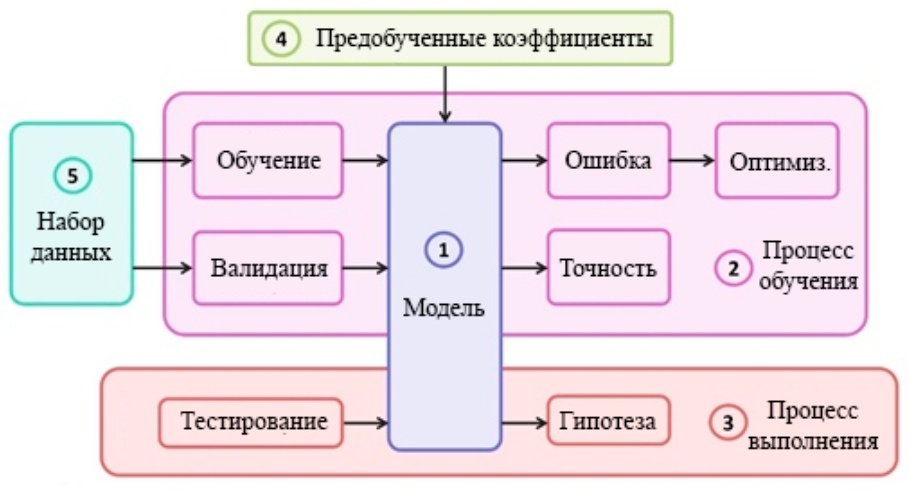
\includegraphics[width=\textwidth]{image020.jpg}
\caption{Иллюстрация подхода дообучения сети}%
\label{fig:how-to-do-research}
\end{figure}

В рамках данной работы были реализованы программы дообучения модели на стационарном устройстве и запуска этой модели на встраиваемом устройстве в режиме реального времени. Также составлены наборы данных для дообучения модели и тестирования. Для решения поставленной задачи был выбран итеративный подход к дообучению сети. Если по результатам эксперимента не была достигнута желаемая точность, то дообучение производится повторно с другим набором данных, или с другими параметрами. 

%%%%%%%%%%%%%%%%%%%%%%%%%%%%%%%%%%%%%%%%%%%%%%%%%%%%%%%%%%%%%%%%%%%%%%%%%%%%%%%%
\section{Программа дообучения модели}
%%%%%%%%%%%%%%%%%%%%%%%%%%%%%%%%%%%%%%%%%%%%%%%%%%%%%%%%%%%%%%%%%%%%%%%%%%%%%%%%

Программа дообучения создана для получения более устойчивой модели обнаружения и расширения множества классифицируемых типов транспортных средств. За основу программы были взяты обучающие примеры из официального репозитория TensorFlow\cite{seventeen}. На рис.~\ref{fig:transferlearningscheme} представлена блок-схема алгоритма дообучения:

\begin{figure}[htbp]
\centering
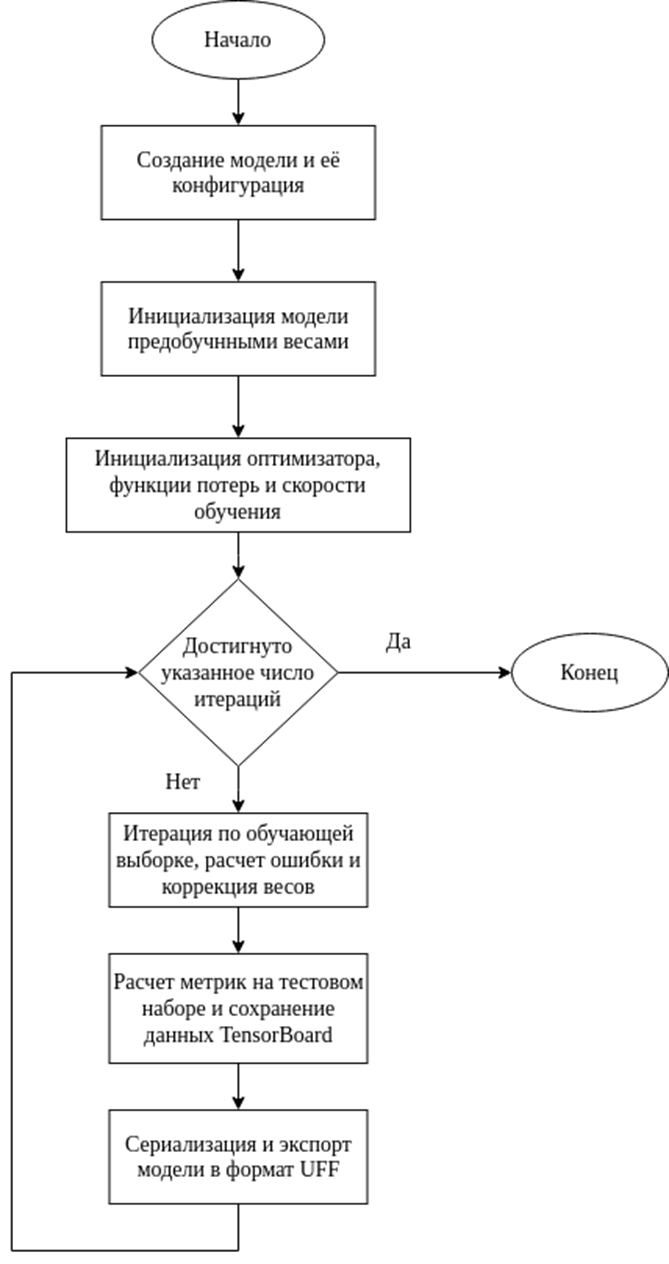
\includegraphics[width=0.75\textwidth]{image021.png}
\caption{Блок-схема алгоритма дообучения}%
\label{fig:transferlearningscheme}
\end{figure}

При запуске программы происходит загрузка настроек и параметров из внешнего файла конфигурации. Данный файл содержит настройки системных путей к обучающему и тестовому наборам данных, перечисления для инициализации функции потерь и оптимизатора, а также значения количества итераций (эпох) дообучения и скорости дообучения модели.

После загрузки параметров конфигурации из файла, происходит создание модели обнаружения объектов. На данном этапе задается структура модели: входная и выходная размерности, количество слоев и их типы, а также функции активации. Так как данная программа создавалась с целью дообучения существующей модели, то далее происходит загрузка коэффициентов модели из внешнего файла.

Перед началом дообучения также происходит инициализация оптимизатора одним из допустимых перечислений. Оптимизаторы позволяют ускорить обучение модели. В TensorFlow API доступно несколько встроенных оптимизаторов, один из них — стохастический градиентный спуск. При стандартном (или «пакетном», «batch») градиентном спуске для корректировки параметров модели используется градиент. Градиент обычно считается как сумма градиентов, вызванных каждым элементом обучения. Вектор параметров изменяется в направлении антиградиента с заданным шагом. Поэтому стандартному градиентному спуску требуется один проход по обучающим данным до того, как он сможет менять параметры. При стохастическом (или «оперативном») градиентном спуске значение градиента аппроксимируются градиентом функции стоимости, вычисленном только на одном элементе обучения. Затем параметры изменяются пропорционально приближенному градиенту. Таким образом параметры модели изменяются после каждого объекта обучения. Для больших массивов данных стохастический градиентный спуск может дать значительное преимущество в скорости по сравнению со стандартным градиентным спуском\cite{eighteen}. 

Далее следует рассчет ошибки модели на обучающих данных и последующая корректировка весов. Шаг, с которым веса корректируются за одну итерацию обучения, обусловлен размером заданной скорости обучения. От него зависит как быстро будет достигнут минимум функции ошибки. При задании малой скорости обучения может потребоваться большее количество итераций, а при задании большой скорости — есть вероятность проскочить минимум функции ошибки.

После каждой итерации происходит расчет метрик точности на тестовом наборе данных. Далее, эти метрики сохраняются в специальный файл, что позволяет отслеживать изменение точности и функции ошибки модели во время дообучения в режиме реального времени. В данной работе для анализа этих данных использовался TensorBoard. Такая стратегия позволяет остановить дообучение в любой момент, если есть подозрение на возможное переобучение модели. 

В конце каждой итерации происходит сериализация и сохранение модели в формате UFF. Это позволяет исключить потерю данных в случае программных ошибок при выполнении программы.
\nomenclature{UFF}{Universal File Format}

%%%%%%%%%%%%%%%%%%%%%%%%%%%%%%%%%%%%%%%%%%%%%%%%%%%%%%%%%%%%%%%%%%%%%%%%%%%%%%%%
\section{Процесс создания устойчивой модели для обнаружения объектов}
%%%%%%%%%%%%%%%%%%%%%%%%%%%%%%%%%%%%%%%%%%%%%%%%%%%%%%%%%%%%%%%%%%%%%%%%%%%%%%%%

В данном подразделе описан процесс использования программы дообучения для получения устойчивой модели. Для осуществления поставленной цели было решено использовать итеративную стратегию дообучения. Таким образом, при получении недостаточно точных результатов, дообучение начинается заново, с исходной контрольной точки, но при другой конфигурации параметров обучения.

%%%%%%%%%%%%%%%%%%%%%%%%%%%%%%%%%%%%%%%%%%%%%%%%%%%%%%%%%%%%%%%%%%%%%%%%%%%%%%%%
\subsection{Составление обучающей выборки}
%%%%%%%%%%%%%%%%%%%%%%%%%%%%%%%%%%%%%%%%%%%%%%%%%%%%%%%%%%%%%%%%%%%%%%%%%%%%%%%%

Несмотря на то, что модель детектора уже содержит некоторые типы транспортных средств, которые перечислены в техническом задании, обучающие наборы включают в себя эти классы, так как разрабатываемая система ориентирована на обнаружение этих классов именно в контексте статической камеры для мониторинга дорожного движения. 

Так как заранее неизвестно какой набор данных позволит достичь желаемой точности, то были сформированы следующие обучающие наборы данных:

%
\begin{itemize*}
  \item Содержащий исключительно трамваи и троллейбусы;
  \item Содержащий все классы в равномерной пропорции;
  \item Содержащий только те классы, которые уже присутствуют в исходной модели.
\end{itemize*}
%

Обучающие данные были взяты из следующих источников:
%
\begin{itemize*}
  \item Собственные изображения;
  \item Изображения из набора ImageNet\cite{nineteen}.
\end{itemize*}
%

База данных ImageNet — проект по созданию и сопровождению массивной базы данных аннотированных изображений, предназначенная для отработки и тестирования методов распознавания образов и машинного зрения. По состоянию на 2016 год в базу данных было записано около десяти миллионов URL с изображениями, которые прошли ручную аннотацию для ImageNet, в аннотациях перечислялись объекты, попавшие на изображение, и прямоугольники с их координатами. База данных с аннотацией и URL изображений от третьих лиц доступна непосредственно через ImageNet, но при этом сами изображения не принадлежат проекту.
\nomenclature{URL}{Uniform Resource Locator}

На рис.~\ref{fig:datasubsetproportions} представлены пропорции, в которых содержатся определенные классы в обучающих наборах.

\begin{figure}[htbp]
\centering
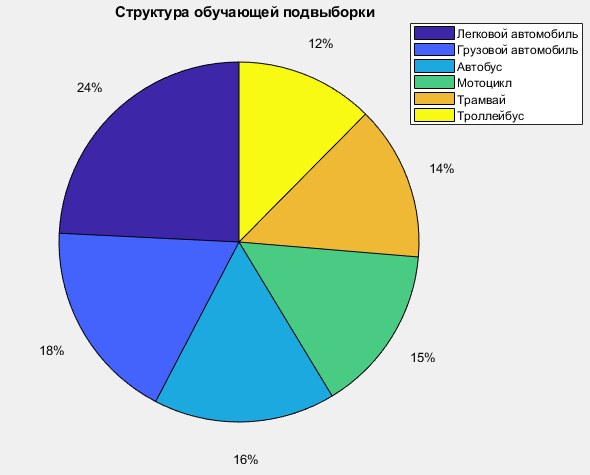
\includegraphics[width=0.85\textwidth]{image022.png}
\caption{Соотношение классов в обучающем наборе}%
\label{fig:datasubsetproportions}
\end{figure}

%%%%%%%%%%%%%%%%%%%%%%%%%%%%%%%%%%%%%%%%%%%%%%%%%%%%%%%%%%%%%%%%%%%%%%%%%%%%%%%%
\subsection{Дообучение модели обнаружения транспортных средств}
%%%%%%%%%%%%%%%%%%%%%%%%%%%%%%%%%%%%%%%%%%%%%%%%%%%%%%%%%%%%%%%%%%%%%%%%%%%%%%%%

Для проведения дообучения использовался API предоставленный в официальном репозитории TensorFlow\cite{twenty}. Репозиторий содержит множество обученных моделей детекторов разных архитектур. Доступны скрипты для обучения модели, конвертации модели и обучающего набора, а также для оценки точности модели на одном из таких наборов как COCO, ImageNet или PascalVOC. Для начала обучения модель необходимо:
%
\begin{itemize*}
  \item Установить зависимости для проекта;
  \item Загрузить предобученную модель (при условии дообучения);
  \item Разделить обучающий набор на подвыборки для обучения, тестирования и оценки;
  \item Сформировать файл с метками классов.
\end{itemize*}
%

После этого можно приступить к началу дообучения выбранной модели.

%%%%%%%%%%%%%%%%%%%%%%%%%%%%%%%%%%%%%%%%%%%%%%%%%%%%%%%%%%%%%%%%%%%%%%%%%%%%%%%%
\subsubsection{Расчет метрик и функции потерь}
%%%%%%%%%%%%%%%%%%%%%%%%%%%%%%%%%%%%%%%%%%%%%%%%%%%%%%%%%%%%%%%%%%%%%%%%%%%%%%%%

Метрики используются для оценки точности модели. Для оценки точности необходимо наличие истинных координат объекта, а также полученных в результате работы модели. 

Точность (precision) и полнота (recall) являются метриками, которые используются при оценке алгоритмов классификации и обнаружения. Точность системы в пределах класса – это доля результатов, действительно принадлежащих данному классу или данной области относительно всех результатов, которые система отнесла к этому классу или области. Полнота системы – это доля найденных системой результатов, принадлежащих классу, относительно всех объектов этого класса в тестовой выборке.

Если 

%
\begin{itemize*}
  \item TP — истинно-положительное решение;
  \item TN — истинно-отрицательное решение;
  \item FP — ложно-положительное решение;
  \item FN — ложно-отрицательное решение, тогда:
\end{itemize*}
%
\begin{center}
Точность \(= \frac{TP}{TP+FP}\)
\end{center}

\begin{center}
Полнота \( = \frac{TP}{TP+FN}\)
\end{center}

%
\begin{itemize*}
  \item Средняя точность (AP) в зависимости от пересечения:
	%
	\begin{itemize*}
	  \item При пересечении областей не менее 50\%;
	  \item При пересечении областей не менее 75\%;
	  \item При пересечении областей не менее 90\%.
	\end{itemize*}
	%
  \item Средняя точность (AP) в зависимости от размера области:
  	%
	\begin{itemize*}
	  \item При размере областей менее \(32^2\);
	  \item При размере областей более \(32^2\) но менее \(96^2\);
	  \item При размере областей более \(96^2\).
	\end{itemize*}
	%
  \item Средняя полнота (AR):
  	%
	\begin{itemize*}
	  \item При максимальном количестве объектов равным 1;
	  \item При максимальном количестве объектов равным 10;
	  \item При максимальном количестве объектов равным 100.
	\end{itemize*}
	%
  \item Средняя полнота (AR) в зависимости от размера области:
  	%
	\begin{itemize*}
	  \item При размере областей менее \(32^2\);
	  \item При размере областей более \(32^2\) но менее \(96^2\);
	  \item При размере областей менее \(96^2\).
	\end{itemize*}
	%
\end{itemize*}
%

Функция потерь — функция, которая характеризует потери при неправильном обнаружении или классификации объекта на основе тестовых данных. При решении задачи классификации - функция потерь является мерой расхождения между истинным значением класса и оценкой класса, полученной с помощью модели.
На рис.~\ref{fig:lossfunctions}  приведены основные типы функций потерь, которые используются в машинном обучении.

\begin{figure}[htbp]
\centering
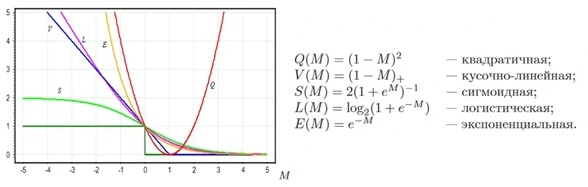
\includegraphics[width=0.85\textwidth]{image025.jpg}
\caption{Иллюстрация зависимостей различных функций потерь\cite{twentyone}}%
\label{fig:lossfunctions}
\end{figure}

При оценке ошибки, в данной работе использовалась сигмоидная функция потерь, так как обладает наименьшим риском привести модель к переобучению при решении задачи обнаружения объектов. 

%%%%%%%%%%%%%%%%%%%%%%%%%%%%%%%%%%%%%%%%%%%%%%%%%%%%%%%%%%%%%%%%%%%%%%%%%%%%%%%%
\subsubsection{Анализ процесса дообучения модели}
%%%%%%%%%%%%%%%%%%%%%%%%%%%%%%%%%%%%%%%%%%%%%%%%%%%%%%%%%%%%%%%%%%%%%%%%%%%%%%%%

С помощью инструмента анализа TensorBoard проводился анализ этапа дообучения модели. После каждой эпохи дообучения делались выводы касательно необходимости продолжения обучения модели. Дообучение прерывалось если было подозрение на достижение моделью этапа переобучения. На рис.~\ref{fig:image026} и ~\ref{fig:image027} можно видеть, как менялась точность модели в зависимости от эпохи дообучения.

\begin{figure}[htbp]
\centering
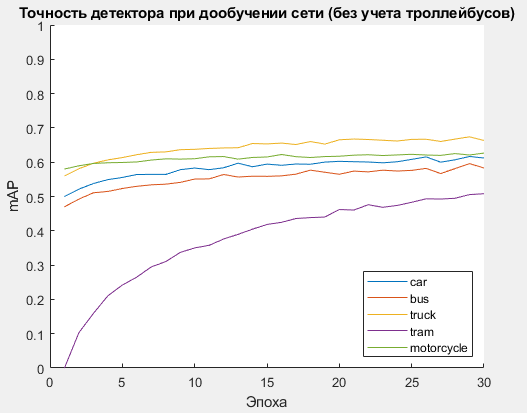
\includegraphics[width=0.85\textwidth]{image026.png}
\caption{Точность модели при дообучении на наборе, содержащем только исходные классы}%
\label{fig:image026}
\end{figure}

На рис.~\ref{fig:lossfunctions} можно наблюдать рост точности обнаружения трамваев и незначительное увеличение точности обнаружения уже имеющихся в модели классов транспортных средств, в пределах 10%. Этот факт можно обосновать наличием в обучающей выборке значительного количества изображений транспортных средств с ракурсов, характерных для положения камер видеомониторинга дорожной ситуации. Помимо этого, все изображения транспортных средств в обучающей выборке имеют черно-белый формат, что отличается от обучающего набора COCO, который состоит, по большей части из цветных изображений. 

При включении в выборку для дообучения метки с классом «троллейбус» можно наблюдать зависимость, представленную на рис.~\ref{fig:image027}.

\begin{figure}[htbp]
\centering
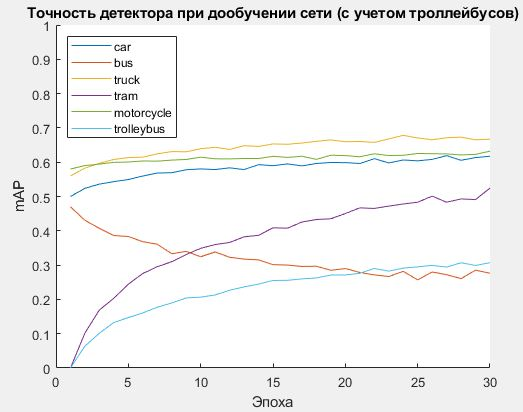
\includegraphics[width=0.85\textwidth]{image027.jpg}
\caption{Точность модели при дообучении на наборе, содержащем все требуемые классы}%
\label{fig:image027}
\end{figure}

Исходя из рис.~\ref{fig:image027} можно сделать вывод о том, что для классов с типом «трамвай» точность обнаружения растет аналогично с предыдущим графиком. Однако, при дообучении с учетом меток типа «троллейбус» можно наблюдать снижение точности обнаружения автобусов. Это объясняется, в первую очередь, низкими интерклассовыми отличиями троллейбусов и автобусов. Также это можно объяснить неспособностью модели правильно выделить ключевые признаки указанных типов транспортных средств. При этом стоит отметить, что наблюдается повышение точности для меток «легковой автомобиль», «грузовой автомобиль» и «мотоцикл» в рамках 10\%, аналогично предыдущей выборке. 

%%%%%%%%%%%%%%%%%%%%%%%%%%%%%%%%%%%%%%%%%%%%%%%%%%%%%%%%%%%%%%%%%%%%%%%%%%%%%%%%
\section{Программа покадрового обнаружения объектов}
%%%%%%%%%%%%%%%%%%%%%%%%%%%%%%%%%%%%%%%%%%%%%%%%%%%%%%%%%%%%%%%%%%%%%%%%%%%%%%%%

Данная программа осуществляет инициализацию модели обнаружения объектов, выполняет покадровую обработку видео из USB-камеры и выводит результаты обнаружения в видеопоток. Данная программа написана с использованием TensorRT API и предназначена для запуска на встраиваемом устройстве Jetson Nano. На рис.~\ref{fig:image028} представлена блок-схема алгоритма программы.

\begin{figure}[htbp]
\centering
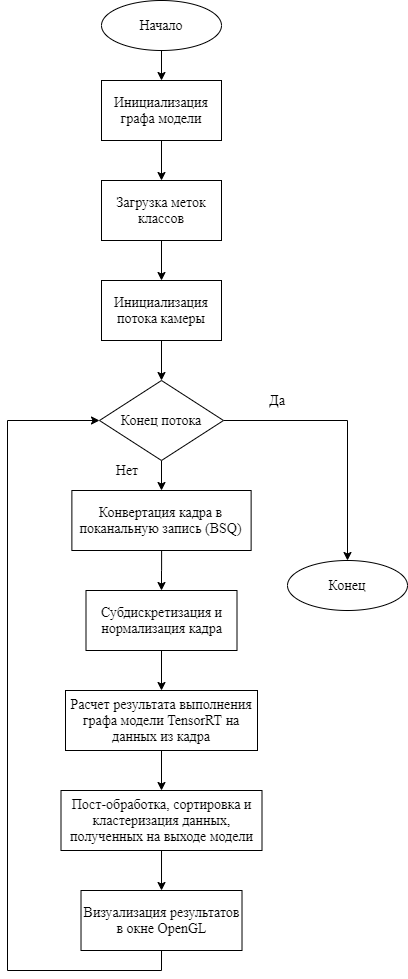
\includegraphics[width=0.60\textwidth]{image028.png}
\caption{Блок-схема алгоритма покадрового обнаружения объектов}%
\label{fig:image028}
\end{figure}

При запуске программы происходит инициализация модели из файла в формате UFF, путь до которого передается в качестве аргумента командной строки. Загрузка меток классов осуществляется из текстового файла, где построчно перечислены все классы, которые обучена определять модель. Также, предварительно производится инициализация подключения к USB-камере, из которого извлекаются кадры для обнаружения объектов.

Для визуализации результатов обнаружения используется библиотека OpenGL, с помощью которой создается окно куда выводится видеопоток. В дальнейшем, с помощью этой библиотеки возможно также перенаправить поток вывода на отдельный порт устройства.

В отличие от программы дообучения, здесь не производится предварительного создания структуры модели до загрузки весов. Вместо этого, TensorRT позволяет создавать и инициализировать модель сразу из графа в формате TensorRT Engine. Однако для использования такого подхода необходимо предварительно осуществить парсинг графа модели из файла UFF.

%%%%%%%%%%%%%%%%%%%%%%%%%%%%%%%%%%%%%%%%%%%%%%%%%%%%%%%%%%%%%%%%%%%%%%%%%%%%%%%%
\subsection{Парсер графа модели из формата UFF}
%%%%%%%%%%%%%%%%%%%%%%%%%%%%%%%%%%%%%%%%%%%%%%%%%%%%%%%%%%%%%%%%%%%%%%%%%%%%%%%%

Парсинг UFF файла осуществляется встроенными средствами TensorRT. При запуске парсера первым делом осуществляется проверка на совместимость версий TensorFlow и TensorRT. В случае если версия TensorFlow сильно опережает TensorRT — в исходном UFF файле могут попадаться функции активации или слои, которые не могут быть обработаны парсером. В таких случаях могут требоваться дополнительные изменения в структуре модели. На табл.~\ref{tabular:tab_tf_trt} представлены совместимые версии TensorFlow и TensorRT.

\begin{table}[H]
	\caption{Соответствие версий TensorFlow и TensorRT}
	\begin{center}
		\begin{tabular}{|l|l|}
			\hline
			Версия TensorFlow & Версия TensorRT\\ \hline
			1.14 & 7.x.x\\ \hline
			1.13 & 7.x.x, 6.x.x\\ \hline
			1.12 & 6.x.x\\ \hline
			1.11 & 5.x.x\\ \hline
		\end{tabular}
		\label{tabular:tab_tf_trt}
	\end{center}
\end{table}

В случае если версии совместимы, то программа десериализует TensorFlow модель и начнет просчитывать наиболее оптимальный вариант конвертации в TensorRT. 

Имеется возможность при вызове парсера указать желаемые оптимизации модели. Оптимизации могут включать в себя объединение слоев и понижение точности весовых коэффициентов. 

Модель в TensorRT представляет из себя план выполнения и состоит из последовательности команд для расчета результата модели. Программа строит план выполнения итерационным методом, пока не будут минимизированы затраты по времени и сложности. Таким образом, во время конвертации происходит перебор возможных комбинаций выполнения процедур свертки и активации, а также замена смежных слоев одним слоем. План выполнения может не отражать реальную структуру модели, а являться приближенным вариантом её расчета, оптимизированным под конкретное устройство и окружение. 

После завершения выполнения конвертации на выходе имеется TensorRT Engine файл, содержащий готовый к выполнению оптимизированный план расчета модели.

%%%%%%%%%%%%%%%%%%%%%%%%%%%%%%%%%%%%%%%%%%%%%%%%%%%%%%%%%%%%%%%%%%%%%%%%%%%%%%%%
\subsection{Получение кадра из потока камеры}
%%%%%%%%%%%%%%%%%%%%%%%%%%%%%%%%%%%%%%%%%%%%%%%%%%%%%%%%%%%%%%%%%%%%%%%%%%%%%%%%

В устройстве Jetson Nano имеется несколько USB-портов, один из которых используется в данной работе для подключения камеры. Такой вариант подключения позволяет получать кадры с помощью библиотеки Gstreamer, которая является частью пакета Jetpack, описанного в подразделе 1.4.3. 

Выбор библиотеки Gstreamer обусловлен также её возможностью использования аппаратной поддержки на Jetson Nano, что позволяет осуществлять декодирование видео с минимальной задержкой.

Для корректной инициализации видеопотока камеры необходимо передать в Gstreamer наименование USB-порта, к которому подключена камера, а также выходное разрешение камеры. Далее программа обнаружения будет брать новый кадр из видеопотока до тех пор, пока поток не будет закрыт или принудительно остановлен.

%%%%%%%%%%%%%%%%%%%%%%%%%%%%%%%%%%%%%%%%%%%%%%%%%%%%%%%%%%%%%%%%%%%%%%%%%%%%%%%%
\subsection{Пост-обработка результатов выполнения модели}
%%%%%%%%%%%%%%%%%%%%%%%%%%%%%%%%%%%%%%%%%%%%%%%%%%%%%%%%%%%%%%%%%%%%%%%%%%%%%%%%

После того как был получен кадр из видеопотока, он передается на вход модели обнаружения и обрабатывается с согласно плану выполнения построенному TensorRT. На выходе получаются множество областей, содержащих координаты и метки классов. 

Первоначальная фильтрация результатов заключается в отсеивании всех гипотез с пустыми метками классов, а также гипотез с уровнем достоверности ниже требуемого (передается в качестве аргумента командной строки). Далее, результаты обнаружения кластеризуются для объединения пересекающихся областей в единую область. При кластеризации, осуществляется итерация по всем гипотезам и для каждой считается площадь пересечения с другими гипотезами. В случае если отношение площади пересечения выше порогового — то области объединяются в одну. При несовпадении меток классов — учитывается только метка класса с более высоким уровнем достоверности. При кластеризации также учитывается не только пересечение областей, но также и отношение этих областей. В случае если области полностью пересекаются, но одна область значительно меньше другой, и, при этом, у областей отличаются метки классов — то такие области не будут объединены в одну, чтобы учитывать возможность наслоения объектов на изображении (например, если мотоцикл стоит на фоне автобуса).

%%%%%%%%%%%%%%%%%%%%%%%%%%%%%%%%%%%%%%%%%%%%%%%%%%%%%%%%%%%%%%%%%%%%%%%%%%%%%%%%
\subsection{Дополнительная классификация меток с типом «автобус»}
%%%%%%%%%%%%%%%%%%%%%%%%%%%%%%%%%%%%%%%%%%%%%%%%%%%%%%%%%%%%%%%%%%%%%%%%%%%%%%%%

В данной работе используется экстрактор признаков InceptionV2, который необходим для классификации и обнаружения объектов. В ходе дообучения модели было выявлено, что классификация троллейбусов выполняется недостаточно точно. Схожесть признаков троллейбуса и автобуса приводит к снижению точности классификации обоих типов транспортных средств. Это связано с тем, что модель не может правильно выделить ключевые признаки этих типов транспорта при дообучении. 

\begin{figure}[htbp]
\centering
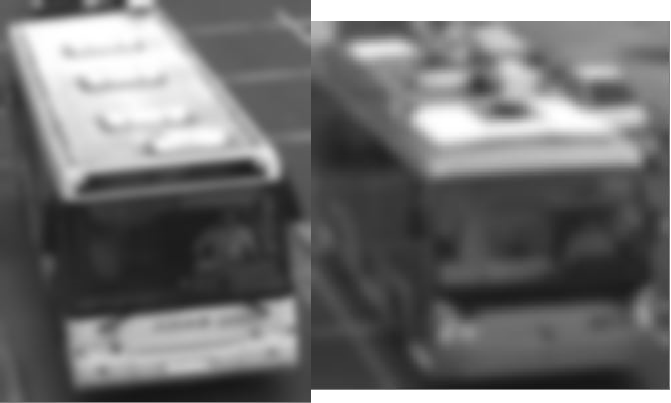
\includegraphics[width=0.95\textwidth]{image029.png}
\caption{Изображения автобуса и троллейбуса после свертки}%
\label{fig:empty}
\end{figure}

Для устойчивой классификации объектов типа «автобус» и «троллейбус» был написан метод дополнительной классификации. Вместо дообучения на наборе, содержащем изображения троллейбусов, решено отдельно производить классификацию с помощью дескрипторов ключевых точек для всех меток «автобус» с целью определения класса принадлежности этого объекта.

Дескриптор – описание особой точки, определяющее особенности её окрестности, представляет собой числовой или бинарный вектор определенных параметров. Длина вектора и вид параметров определяются применяемым алгоритмом.  Дескриптор позволяет выделить особую точку из всего их множества на изображении, это необходимо для составления ключевых пар особенностей, принадлежащих одному объекту, при сравнении разных изображений\cite{twentytwo}.

В качестве области потенциальных ключевых точек была выбрана зона верхней части транспортного средства, на которой расположены устройства для подключения к энергосети. 

\begin{figure}[htbp]
\centering
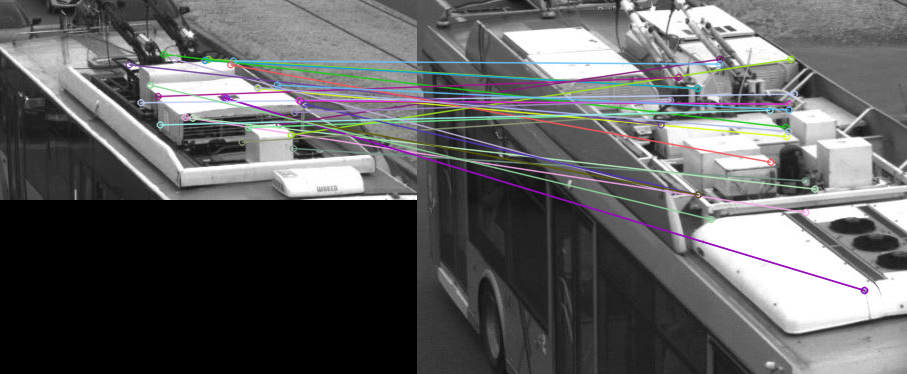
\includegraphics[width=0.95\textwidth]{image030.png}
\caption{Поиск ключевых точек троллейбуса}%
\label{fig:empty}
\end{figure}

Предварительно, перед началом обработки изображения на наличие ключевых точек, производилась фильтрация изображения фильтром Лапласа или алгоритмом Кэнни для выделения контуров. Для корректного нахождения и расчёта дескрипторов ключевых точек этой зоны тестировались различные подходы: 

%
\begin{itemize*}
  \item ORB;
  \item BRISK;
  \item AKAZE.
\end{itemize*}
%

%%%%%%%%%%%%%%%%%%%%%%%%%%%%%%%%%%%%%%%%%%%%%%%%%%%%%%%%%%%%%%%%%%%%%%%%%%%%%%%%
\subsubsection{ORB}
%%%%%%%%%%%%%%%%%%%%%%%%%%%%%%%%%%%%%%%%%%%%%%%%%%%%%%%%%%%%%%%%%%%%%%%%%%%%%%%%

ORB представлен в 2011 году\cite{twentytwo}. В его основе лежит комбинация таких алгоритмов как детектор FAST (Features from Accelerated Segment Test) и дескриптор BRIEF (Binary Robust Independent Elementary Features) с некоторыми улучшениями. 

Первым делом используется FAST для нахождения ключевых точек, после чего применяется детектор углов Харриса для определения \(N\) наиболее успешных кандидатов среди этих точек. Для обеспечения инвариантности относительно угла поворота рассчитывается градиент интенсивности в окружности радиуса \(R\) с центром в ключевой точке.

Для расчета дескриптора ключевой точки используется алгоритм BRIEF. Этот алгоритм строит вектор из \(M\) бинарных сравнений по интенсивности пикселей в окружности с ключевой точкой в центре. Для обеспечения инвариантности относительно угла поворота области используется ранее вычисленный градиент.

%%%%%%%%%%%%%%%%%%%%%%%%%%%%%%%%%%%%%%%%%%%%%%%%%%%%%%%%%%%%%%%%%%%%%%%%%%%%%%%%
\subsubsection{BRISK}
%%%%%%%%%%%%%%%%%%%%%%%%%%%%%%%%%%%%%%%%%%%%%%%%%%%%%%%%%%%%%%%%%%%%%%%%%%%%%%%%

Целью создания данного метода было достижение инвариантности к изменению масштаба, при этом сохранив высокую скорость работы. Авторы метода создали свой метод на основе детектора AGAST, который, по сути, является расширением метода FAST\cite{twentytwo}. Однако для того, чтобы добиться инвариантности к изменению масштаба, нахождение максимумов происходит не только на исходном изображении, но и в масштабируемом пространстве. В методе BRISK масштабируемое пространство состоит из \(n\) октав \(c_i\) и \(n\) внутренних октав \(d_i\), \(i = {0, 1, ..., n-1}\). \(n\) обычно выбирается равным 4. Октавы составляются путём уменьшения масштаба исходного изображения в два раза. Каждая внутренняя октава \(d_i\) располагается между октавами \(c_i\) и \(c_{i+1}\). Первая внутренняя октава получается путём уменьшения масштаба исходного изображения в 1.5 раза, а каждая последующая — путём уменьшения масштаба предыдущей внутренней октавы в два раза.

Метод FAST применяется к каждой из октав и каждой из внутренних октав по отдельности с одинаковым пороговым значением, с целью найти потенциально особые области. Затем среди точек, содержащихся в этих областях, производится поиск локальных максимумов во всём масштабируемом пространстве.

%%%%%%%%%%%%%%%%%%%%%%%%%%%%%%%%%%%%%%%%%%%%%%%%%%%%%%%%%%%%%%%%%%%%%%%%%%%%%%%%
\subsubsection{AKAZE}
%%%%%%%%%%%%%%%%%%%%%%%%%%%%%%%%%%%%%%%%%%%%%%%%%%%%%%%%%%%%%%%%%%%%%%%%%%%%%%%%

При разработке данного метода, представленного в 2013 году, старались добиться высокой скорости работы как детектора, так и дескриптора\cite{twentytwo}. При этом найденные особые точки и их дескрипторы должны были удовлетворять высоким показателям точности при сравнении изображений.

Применение алгоритма FED - Fast Explicit Diffusion на пирамидальной схеме позволяет построить нелинейную многомасштабную пирамиду. Применение нелинейного коэффициента масштабирования позволяет увеличить скорость нахождения нужной особой точки по сравнению с Гауссовой пирамидой, так как вычисление данного коэффициента основано на изменении яркости изображения при масштабировании.

Детектор особых точек работает следующим образом. Для каждого октавы \(L_i\) в пирамиде вычисляется определитель Гессиана. Производные второго порядка вычисляются с помощью фильтра Шарра. Данный фильтр позволяет учитывать ориентацию особых точек. С помощью такого подхода ищем такие точки в октаве, значение фильтра которых выше заданного порога и является наибольшим из окрестности точки \(3*3\) пикселей.

Далее, для каждой точки из потенциальных максимумов сравнивается её значение относительно результатов в соседних октавах \(i+1\) и \(i-1\) в окне размером \(\sigma_i * \sigma_i\) соответственно. В итоге расположение особой точки оценивается с субпиксельной точностью соответствуя квадратичной функции к определителю Гессиана в \(3*3\) соседних пикселей для поиска максимума.

Далее происходит вычисление дескрипторов. Первоначальный дескриптор LDB основывался на тех же принципах что и рассмотренный выше BRIEF, но к сравнениям яркостных показателей областей добавили сравнение значений градиентов яркости по оси \(x\) и \(y\), в итоге результат одного теста состоит из трех битов вместо одного. Проведение тестов проводилось в окне размером \(20*20\) пикселей, деленном на 4, 9 и 16 областей.

Но LDB имеет недостатки такие как не инвариантность к вращению и масштабированию. И в качестве решения этих проблем в AKAZE используется его улучшенная версия – M-LDB:
%
\begin{itemize*}
  \item Окно дескриптора ориентируется по ориентации особой точки;
  \item Инвариантность к масштабу получена с помощью выбора размера окна дескриптора в зависимости от размера октавы \(\sigma_i\) в которой найдена его особая точка.
\end{itemize*}
%

В отличии от LDB в M-LDB тесты проводятся не между средним значением всех пикселей в области, а между заданным их количеством в зависимости от размера \(\sigma_i\). Что позволяет ускорить вычисление дескриптора. Итоговый бинарный дескриптор имеет длину 486 по три составляющих.

%%%%%%%%%%%%%%%%%%%%%%%%%%%%%%%%%%%%%%%%%%%%%%%%%%%%%%%%%%%%%%%%%%%%%%%%%%%%%%%%
\section{Выводы по разделу}
%%%%%%%%%%%%%%%%%%%%%%%%%%%%%%%%%%%%%%%%%%%%%%%%%%%%%%%%%%%%%%%%%%%%%%%%%%%%%%%%

В данном разделе описаны основные компоненты системы обнаружения и классификации транспортных средств. Приведены блок-схемы алгоритмов дообучения и обнаружения, а также описан процесс дообучения модели, Реализованы программы дообучения модели на стационарном устройстве и запуска этой модели на встраиваемом устройстве в режиме реального времени. Также составлены наборы данных для дообучения модели и тестирования. Для решения поставленной задачи был выбран итеративный подход к дообучению сети. Если по результатам эксперимента не была достигнута желаемая точность, то дообучение производилось повторно с другим набором данных, или с другими параметрами. 

По результатам процесса дообучения можно наблюдать рост точности обнаружения трамваев и незначительное увеличение точности обнаружения уже имеющихся в модели классов транспортных средств, в пределах 10\%. Этот факт можно обосновать наличием в обучающей выборке значительного количества изображений транспортных средств с ракурсов, характерных для положения камер видеомониторинга дорожной ситуации. 

Для устойчивой классификации объектов типа «автобус» и «троллейбус» написан метод дополнительной классификации. Отдельно произведена классификация с помощью дескрипторов ключевых точек для всех меток «автобус» с целью определения класса принадлежности этого объекта. Протестированы различные методы обнаружения ключевых точек – ORB, BRISK, AKAZE.

\iffalse
%%%%%%%%%%%%%%%%%%%%%%%%%%%%%%%%%%%%%%%%%%%%%%%%%%%%%%%%%%%%%%%%%%%%%%%%%%%%%%%%
\section{0xDEADBEEF}
%%%%%%%%%%%%%%%%%%%%%%%%%%%%%%%%%%%%%%%%%%%%%%%%%%%%%%%%%%%%%%%%%%%%%%%%%%%%%%%%

\Blindtext

%%%%%%%%%%%%%%%%%%%%%%%%%%%%%%%%%%%%%%%%%%%%%%%%%%%%%%%%%%%%%%%%%%%%%%%%%%%%%%%%
\section{0xC0DECAFE}
%%%%%%%%%%%%%%%%%%%%%%%%%%%%%%%%%%%%%%%%%%%%%%%%%%%%%%%%%%%%%%%%%%%%%%%%%%%%%%%%

You can review what you have to do in figure~\ref{fig:how-to-do-research}.
Please do so now. \blindtext

\Blindtext
\fi